%----------------------------------------------------------------------------------------
%	PACKAGES AND OTHER DOCUMENT CONFIGURATIONS
%----------------------------------------------------------------------------------------

\documentclass{article}

\usepackage{fancyhdr} % Required for custom headers
\usepackage{lastpage} % Required to determine the last page for the footer
\usepackage{extramarks} % Required for headers and footers
\usepackage[usenames,dvipsnames]{color} % Required for custom colors
\usepackage{pgf} % Required to insert pgf plots from matplotlib
\usepackage{graphicx} % Required to insert images
\usepackage{listings} % Required for insertion of code
\usepackage{courier} % Required for the courier font
\usepackage{lipsum} % Used for inserting dummy 'Lorem ipsum' text into the template
\usepackage[utf8]{inputenc}
\usepackage[ngerman]{babel}

% Margins
\topmargin=-0.45in
\evensidemargin=0in
\oddsidemargin=0in
\textwidth=6.5in
\textheight=9.0in
\headsep=0.25in

\linespread{1.1} % Line spacing

% Set up the header and footer
\pagestyle{fancy}
%\lhead{\hmwkAuthorName} % Top left header
\chead{\hmwkClass\ : \hmwkTitle} % Top center head
\rhead{\firstxmark} % Top right header
\lfoot{\lastxmark} % Bottom left footer
\cfoot{} % Bottom center footer
\rfoot{Page\ \thepage\ of\ \protect\pageref{LastPage}} % Bottom right footer
\renewcommand\headrulewidth{0.4pt} % Size of the header rule
\renewcommand\footrulewidth{0.4pt} % Size of the footer rule

\setlength\parindent{0pt} % Removes all indentation from paragraphs

%----------------------------------------------------------------------------------------
%	CODE INCLUSION CONFIGURATION
%----------------------------------------------------------------------------------------

\definecolor{MyDarkGreen}{rgb}{0.0,0.4,0.0} % This is the color used for comments
\lstloadlanguages{Perl} % Load Perl syntax for listings, for a list of other languages supported see: ftp://ftp.tex.ac.uk/tex-archive/macros/latex/contrib/listings/listings.pdf
\lstset{language=Perl, % Use Perl in this example
        frame=single, % Single frame around code
        basicstyle=\small\ttfamily, % Use small true type font
        keywordstyle=[1]\color{Blue}\bf, % Perl functions bold and blue
        keywordstyle=[2]\color{Purple}, % Perl function arguments purple
        keywordstyle=[3]\color{Blue}\underbar, % Custom functions underlined and blue
        identifierstyle=, % Nothing special about identifiers                                         
        commentstyle=\usefont{T1}{pcr}{m}{sl}\color{MyDarkGreen}\small, % Comments small dark green courier font
        stringstyle=\color{Purple}, % Strings are purple
        showstringspaces=false, % Don't put marks in string spaces
        tabsize=5, % 5 spaces per tab
        %
        % Put standard Perl functions not included in the default language here
        morekeywords={rand},
        %
        % Put Perl function parameters here
        morekeywords=[2]{on, off, interp},
        %
        % Put user defined functions here
        morekeywords=[3]{test},
       	%
        morecomment=[l][\color{Blue}]{...}, % Line continuation (...) like blue comment
        numbers=left, % Line numbers on left
        firstnumber=1, % Line numbers start with line 1
        numberstyle=\tiny\color{Blue}, % Line numbers are blue and small
        stepnumber=5 % Line numbers go in steps of 5
}

% Creates a new command to include a perl script, the first parameter is the filename of the script (without .pl), the second parameter is the caption
\newcommand{\perlscript}[2]{
\begin{itemize}
\item[]\lstinputlisting[caption=#2,label=#1]{#1.pl}
\end{itemize}
}

%----------------------------------------------------------------------------------------
%	DOCUMENT STRUCTURE COMMANDS
%	Skip this unless you know what you're doing
%----------------------------------------------------------------------------------------

% Header and footer for when a page split occurs within a problem environment
\newcommand{\enterProblemHeader}[1]{
%\nobreak\extramarks{#1}{#1 continued on next page\ldots}\nobreak
%\nobreak\extramarks{#1 (continued)}{#1 continued on next page\ldots}\nobreak
}

% Header and footer for when a page split occurs between problem environments
\newcommand{\exitProblemHeader}[1]{
%\nobreak\extramarks{#1 (continued)}{#1 continued on next page\ldots}\nobreak
%\nobreak\extramarks{#1}{}\nobreak
}

\setcounter{secnumdepth}{0} % Removes default section numbers
\newcounter{homeworkProblemCounter} % Creates a counter to keep track of the number of problems

\newcommand{\homeworkProblemName}{}
\newenvironment{homeworkProblem}[1][Problem \arabic{homeworkProblemCounter}]{ % Makes a new environment called homeworkProblem which takes 1 argument (custom name) but the default is "Problem #"
\stepcounter{homeworkProblemCounter} % Increase counter for number of problems
\renewcommand{\homeworkProblemName}{#1} % Assign \homeworkProblemName the name of the problem
\section{\homeworkProblemName} % Make a section in the document with the custom problem count
%\enterProblemHeader{\homeworkProblemName} % Header and footer within the environment
}{
%\exitProblemHeader{\homeworkProblemName} % Header and footer after the environment
}

\newcommand{\problemAnswer}[1]{ % Defines the problem answer command with the content as the only argument
\noindent\framebox[\columnwidth][c]{\begin{minipage}{0.98\columnwidth}#1\end{minipage}} % Makes the box around the problem answer and puts the content inside
}

\newcommand{\homeworkSectionName}{}
\newenvironment{homeworkSection}[1]{ % New environment for sections within homework problems, takes 1 argument - the name of the section
\renewcommand{\homeworkSectionName}{#1} % Assign \homeworkSectionName to the name of the section from the environment argument
\subsection{\homeworkSectionName} % Make a subsection with the custom name of the subsection
%\enterProblemHeader{\homeworkProblemName\ [\homeworkSectionName]} % Header and footer within the environment
}{
%\enterProblemHeader{\homeworkProblemName} % Header and footer after the environment
}

%----------------------------------------------------------------------------------------
%	NAME AND CLASS SECTION
%----------------------------------------------------------------------------------------

\newcommand{\hmwkTitle}{Übung\ \#3} % Assignment title
\newcommand{\hmwkDueDate}{Montag,\ 10.\ November\ 2014} % Due date
\newcommand{\hmwkClass}{Introduction to HPC} % Course/class
\newcommand{\hmwkClassTime}{} % Class/lecture time
\newcommand{\hmwkClassInstructor}{} % Teacher/lecturer
\newcommand{\hmwkAuthorName}{Günther Schindler, Christoph Klein, Klaus Naumann} % Your name

%----------------------------------------------------------------------------------------
%	TITLE PAGE
%----------------------------------------------------------------------------------------

\title{
\vspace{2in}
\textmd{\textbf{\hmwkClass:\ \hmwkTitle}}\\
\normalsize\vspace{0.1in}\small{Abgabe\ am\ \hmwkDueDate}\\
\vspace{0.1in}\large{\textit{\hmwkClassTime}}
\vspace{3in}
}

\author{\textbf{\hmwkAuthorName}}
\date{} % Insert date here if you want it to appear below your name

%----------------------------------------------------------------------------------------

\begin{document}

\maketitle

%----------------------------------------------------------------------------------------
%	TABLE OF CONTENTS
%----------------------------------------------------------------------------------------

%\setcounter{tocdepth}{1} % Uncomment this line if you don't want subsections listed in the ToC

\newpage
\tableofcontents
\newpage

%----------------------------------------------------------------------------------------
%	Moores Law
%----------------------------------------------------------------------------------------

% To have just one problem per page, simply put a \clearpage after each problem

\begin{homeworkProblem}[Moores Law]
\subsection{Apply Moore's Law}
As part of the third exercise we should apply Moore's Law to the currently fastest
supercomputer worldwide and predict the achievement of one Exaflop.
\\
According to the list of june 2014 published on www.top500.org the currently fastest
supercomputer worldwide is Tianhe-2, a supercomputer developed by China's National
University of Defense Technology. It has a performance of 33.86 Pflop/s on the
Linpack benchmark.
\\
In the mid 1960s Gordon Moore made the observation that computer power, measured by the 
number of transistors that could be fit onto a chip, doubled once every 18 months. This
law can be stated in mathematical terms as
\\\\
$K_{(t)} = K_{0} \cdot 2^{t/T_{2}}$ ,
\\\\
where K is the computer power at the reference year t and $T_{2}$ (= 18 months) is time 
for duplication. After reorganizing we get
\\\\
t = $\frac{T_{2} \cdot ln(K_{(t)} / K_{0})}{ln(2)}$ .
\\\\
Based on the 33.86 Pflop/s of Tianhe-2 we predict
\\\\
$\Delta t = \frac{18 \cdot ln(1000 / 33.86)}{ln(2)} \approx 87.91 Month \approx 7.33 Years $
\\\\
to exceed the Exaflop performance (2021).
%\begin{lstlisting}{c}
%\end{lstlisting}

\end{homeworkProblem}
\clearpage
%----------------------------------------------------------------------------------------
%	Amdahl's Law
%----------------------------------------------------------------------------------------
\begin{homeworkProblem}[Amdahl's Law]
\begin{equation}
Speedup = \frac{1}{(1 - P) + \frac{P}{N}}
\end{equation}

\textbf{Part 1:} \\
\begin{equation}
Speedup = \frac{1}{(1 - 0.4) + \frac{0.4}{10}} = \frac{1}{0.6 + 0.04} = 1.5625
\end{equation}
According to Amdahl's law the Speedup is 1.5625. \\

\textbf{Part 2:} \\ \\
Possibility 1: \\
\begin{equation}
Speedup = \frac{1}{(1 - 0.2) + \frac{0.2}{10}} = \frac{1}{0.8 + 0.02} = 1.2195
\end{equation}
Possibility 2: \\
\begin{equation}
Speedup = \frac{1}{(1 - 0.5) + \frac{0.5}{1.6}} = \frac{1}{0.5 + 0.3125} = 1.2308
\end{equation}
As one can see possibility 2 results in an higher speedup and is therefore the optimal solution. \\ \\
\textbf{Part 3:} \\
\begin{equation}
Speedup = \frac{1}{(1 - P) + \frac{P}{N}}
\end{equation}
\begin{equation}
100 = \frac{1}{(1 - P) + \frac{P}{128}}
\end{equation}
\begin{equation}
100 = \frac{128}{128 - 127P}
\end{equation}
\begin{equation}
100(128 - 127P) = 128
\end{equation}
\begin{equation}
P = 0.9978 = 99.78 \%
\end{equation}
\begin{equation}
S = 1 - P = 1 - 0.9978 = 0.0022 = 0.22 \%
\end{equation}
In order to achieve a speedup of 100x, the serial fraction can't be higher than 0.22\%.
\end{homeworkProblem}
\clearpage
%----------------------------------------------------------------------------------------
%	Measure Latency
%----------------------------------------------------------------------------------------
\begin{homeworkProblem}[Measure Latency]
\begin{lstlisting}{c}
#include <iostream>
#include <stdlib.h>
#include "mpi.h"

#define MS 	1024*1024		// define max. message size
using namespace std;

int main(int argc, char** argv)
{
    double 	 *signal;
    int          rank, size, loops;
    double       starttime, endtime, t;
   
    MPI_Init( &argc, &argv );
	
    MPI_Status   status;
    MPI_Request  req;

    MPI_Comm_rank(MPI_COMM_WORLD, &rank);
    MPI_Comm_size(MPI_COMM_WORLD, &size);

    if(size < 2) {
	cout << "Minimum of 2 Processes required! Aborting programm!";
	MPI_Abort(MPI_COMM_WORLD, 1);
    }

    for (int k = 1024; k <= MS; k *= 2) {
	loops = 10;

        signal = (double *) malloc(k * sizeof(double));

            if (rank == 0) {
                /* Synchronize both processes */
		
		MPI_Barrier(MPI_COMM_WORLD); 
                starttime = MPI_Wtime();
                
		for (int j = 0; j < loops; j++) {
		  
                    MPI_Isend( signal, k, MPI_DOUBLE, 1, j, MPI_COMM_WORLD, &req );
                    MPI_Wait( &req, &status );
                    MPI_Irecv( signal, k, MPI_DOUBLE, 1, j, MPI_COMM_WORLD, &req );
                    MPI_Wait( &req, &status );
		    
                }
                endtime = MPI_Wtime();
		t = (endtime - starttime) / loops;
                
            }
            else {
                /* Synchronize both processes */
		
		MPI_Barrier(MPI_COMM_WORLD);
                
		for (int j = 0; j < loops; j++) {
		  
                    MPI_Irecv( signal, k, MPI_DOUBLE, 0, j, MPI_COMM_WORLD, &req );
                    MPI_Wait( &req, &status );
                    MPI_Isend( signal, k, MPI_DOUBLE, 0, j, MPI_COMM_WORLD, &req );
                    MPI_Wait( &req, &status );
		    
                }
            }


        if (rank == 0) {

            cout << "Full round-trip:\t" << k << "\t" << t << endl;
	    cout << "Half round-trip:\t" << k << "\t" << t/2.0 << endl;
	    
        }
    }

    MPI_Finalize( );
    return 0;
}
\end{lstlisting}
\subsection{}
\begin{figure}   
        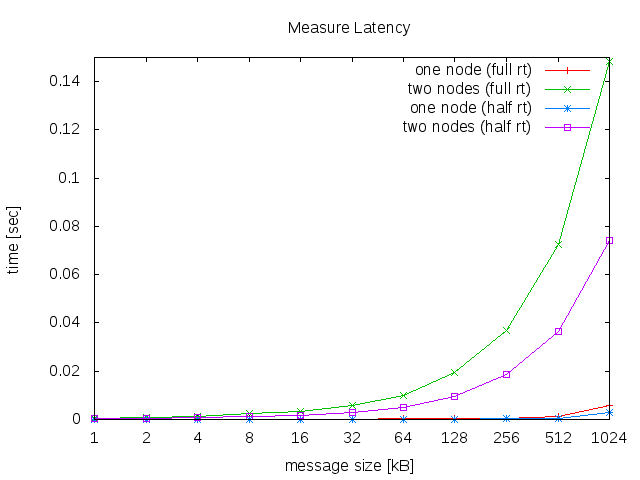
\includegraphics[scale=1.0]{measure_latency.png}
    \caption{Full and Half round-trip latency depending on message sizes from 1 kB to 1024 kB and whether the program is executed on one (with two processes) or two nodes}
\end{figure} 
\subsection{}
As shown in the diagramm \textit{Measure Latency} on the next page both the half round-trip and the full round-trip on two nodes requires more time than both measurements on one node with two processes. The gap between both measurements gets higher with rising message size. A reason for this is a higher intra-node bandwidth compared to two nodes connected through a network. So the sending / receiving time ascends with bigger messages. \\ \\
The latency for the intra-node ping-pong test is about 14 times faster than for the inter-node version for 1024 kB. 
Because of the fact that latency increases for inter-node message parsing it is of primary importance to design algorithms which are efficient and can bridge this latency gap to achieve a high performance.
\end{homeworkProblem}
\clearpage
%----------------------------------------------------------------------------------------
%	Measure Bandwidth
%----------------------------------------------------------------------------------------
\begin{homeworkProblem}[Measure Bandwidth]

\end{homeworkProblem}
\clearpage
\end{document}
